\section{Tomcat : conteneur de servlet Java EE}
%Nicolas
\subsection{Presentation}
\begin{frame}
  \frametitle{Pr�sentation de Tomcat}

  \begin{itemize}
    \item Projet open-source de la fondation Apache
    \item Serveur d'applications Java
    \begin{itemize}
      \item Servlet (g�n�ration de page Html, xml etc...)
      \item JavaServer Pages
    \end{itemize}
    \item 
  \end{itemize}
\end{frame}

\begin{frame}
  \frametitle{Autres serveurs d'applications existants}
En r�alit�, Tomcat esseulement un conteneur de servlets, il existe des serveurs impl�mentant les normes JEE (s�curit�, ejbs, transactions globales...) :
\begin{itemize} 
  \item GlassFish (D�velopp� par Oracle)
  \item jBoss (Utilise Tomcat pour la partie Servlet/JSP)
  \item Websphere (IBM)
  \item ...
\end{itemize}
\end{frame}

\begin{frame}
  \frametitle{Pr�sentation Tomcat
  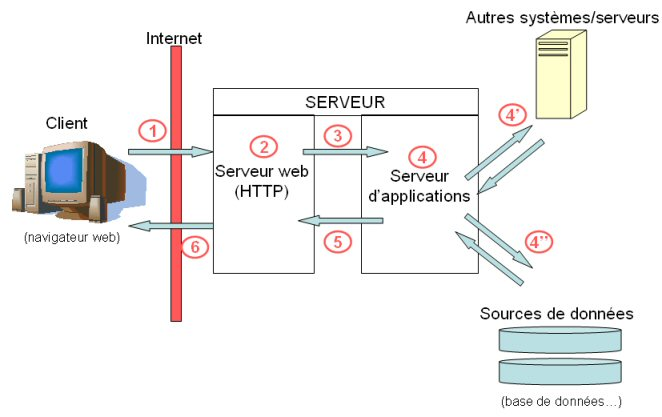
\includegraphics[scale=0.5]{Images/serveurapp.png}
\end{frame}

\subsection{Configuration}
\begin{frame}
  \frametitle{Fichiers de configuration}

		R�pertoire d'installation : CATALINA\_HOME
\begin{itemize} 
    \item \textbf{bin/} ex�cutables de Tomcat(d�marrage du serveur)
    \item \textbf{common/} classes et librairies partag�es par les applications web
    \item \textbf{conf/} Fichiers de configuration
    \item \textbf{Logs/} Logs d'acc�s, erreurs...
    \item \textbf{server/} contient les applications web du serveur en lui-m�me
    \item \textbf{shared/} contient les classes et librairies partag�es par toutes les applications web h�berg�es sur le serveur
    \item \textbf{temp/}
    \item \textbf{webapps/} contient les applications web
    \item \textbf{work/} contient les JSP compil�es
\end{itemize} 
\end{frame}


\begin{frame}
  \frametitle{conf/server.xml}

\begin{itemize}
  \item \$CATALINA\_HOME/server.xml : principal fichier de configuration
  \item El�ments conteneurs (obligatoirs) : Engine, Host, Connector
  \item D�finition des services, protocoles, port utilis�s, redirection vers des ressources externes, des serveurs externes
  \item El�ments facultatifs : GlobalNamingResources, Resources, Realm et Valve.
\end{itemize} 

\begin{lstlisting}
  <Server port="8009" shutdown="SHUTDOWN">
  ...
  </Server>
\end{lstlisting}
		
}


\begin{frame}
  \frametitle{conf/server.xml}
		El�ment Connecteur
		\begin{itemize} 
   		\item objet Java capable d'�couter un port pr�cis et comprenant un protocole pr�cis
    	\item redirige les requ�tes qu'il re�oit au moteur de servlets
      \item C'est l'�l�ment qui re�oit les requ�tes HTTP et les transmet au conteneur de servlet
		\end{itemize}

		\begin{lstlisting}
<Connector port="8080"
	protocol="HTTP/1.1"
	connectionTimeout="20000"
	maxThread="100"
	maxCount="100"
	redirectPort="8443" />
		\end{lstlisting}
\end{frame}

\begin{frame}
    \frametitle{conf/server.xml}
		El�ments Engine et Host
		\begin{itemize}
   		\item \textbf{El�ment Engine} : mod�lise le moteur de servlet, contient un ou plusieurs hosts
    	\item \textbf{El�ment Host} h�te virtuel (Similaire aux virtualhosts d'Apache)
		\end{itemize}

		\begin{lstlisting}
<Engine name="Catalina">
  <Host name="localhost" appBase="webapps"
    unpackWARs="true" autoDeploy="true">
    <!-- contenu de l'�l�ment Host -->
  </Host>
</Engine>
		\end{lstlisting}
\end{frame}

\begin{frame}
  \frametitle{conf/server.xml}
		Resssources et variables d'environnement

		\begin{lstlisting}
<GlobalNamingResources>
  <Resource name="UserDatabase" auth="Container" type="org.apache.catalina.UserDatabase" description="User database that can be updated and saved" factory="org.apache.catalina.users.MemoryUserDatabaseFactory" pathname="conf/tomcat-users.xml" />
  <Environment name="maxRetry" type="java.lang.Integer" value="10" override="false"/>
</GlobalNamingResources>

		\end{lstlisting}
\end{frame}

\subsection{D�ploiement d'une application}
\begin{frame}
\frametitle{Via le manager}
	Installation d'une application web sous la forme d'une archive war
  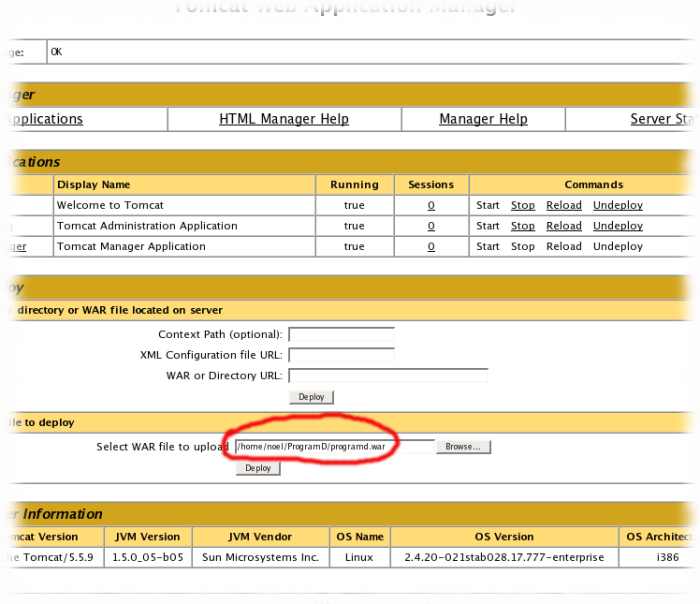
\includegraphics[scale=0.3]{Images/tomcat-deploy-war.png}
\end{frame}

\begin{frame}
  \frametitle{Directement dans le dossier de Tomcat}

  \begin{itemize}
    \item Placer l'archive war dans le dossier webapps/
    \item Tomcat d�compresse l'application au d�marrage
    \item L'application est accessible par l'url http://serveur.tld/nom\_archive\_war
  \end{itemize}
\end{frame}

